%% ICST 2027 -- Research Papers Track
%% Limit: 10 pages including all text, figures, tables and appendices,
%%        plus two additional pages containing ONLY references.
%% Format: two-column IEEE conference publication format, letter template,
%%        conference option.
%% Double-anonymous: no author names, affiliations, acknowledgments or
%%        identifying artifact links anywhere in this file.
\documentclass[10pt,conference,letterpaper]{IEEEtran}
\IEEEoverridecommandlockouts

\usepackage{cite}
\usepackage{amsmath,amssymb}
\usepackage{booktabs}
\usepackage{graphicx}
\usepackage{xcolor}
\usepackage{tikz}
\usetikzlibrary{arrows.meta,positioning,patterns}
\usepackage[hidelinks]{hyperref}

\newcommand{\killk}[1]{Kill@#1}
\definecolor{oaccent}{HTML}{2F5D8C}
\definecolor{ofail}{HTML}{A5372F}
\definecolor{opass}{HTML}{2C6B4D}
\definecolor{orule}{HTML}{B9C2CE}

\begin{document}

\title{Kill Rate Is Not Enough: Selection Inflation and\\
Candidate-Validity Regression in LLM-Based\\
Mutation Test Generation}

\author{\IEEEauthorblockN{}\IEEEauthorblockA{}}

\maketitle

\begin{abstract}
\textbf{Background.} Large language models are increasingly used to generate
unit tests, and mutation kill rate is a common way to score them. Kill rate
alone rewards any candidate that distinguishes a mutant from its reference,
including a test that fails universally.
\textbf{Aims.} We measure how far a development-panel gain transfers to a locked
split, whether kill rate and candidate validity move together under supervised
fine-tuning, and whether a full-scale rehearsal on a permitted split can
establish that an evaluation pipeline computes what it claims.
\textbf{Method.} Four arms of a 1.5B-parameter code model were evaluated under
one frozen generation protocol with eight candidates per target at seed 42, on a
selection panel of 542 function targets. One checkpoint was then evaluated
against the untrained base on a locked split of 757 targets under a promotion
rule committed before either arm ran. A receipt-bound rehearsal re-executed the
entire measurement path at full scale on the permitted panel.
\textbf{Results.} \killk{8} rose from $0.605166$ to $0.695572$ on the selection
panel. On the locked split the paired difference was $+3.4346$ points
($450/757 \to 476/757$; $+114/-88$; net $+26$) with exact two-sided McNemar
$p = 0.0783$ against a predeclared $p < 0.01$, so the base model was retained.
Reference validity fell $11.8726$ points over the same comparison while parse and
execution validity did not regress. The rehearsal reproduced a prior \killk{8}
of $0.605166$ exactly across $4{,}336$ candidates with complete raw-output
integrity.
\textbf{Conclusions.} A selection-panel gain is not evidence of generalization;
a kill-rate-only report can hide a validity regression moving the other way; and
executing the whole measurement path on permitted data at full scale is a
practical precondition for trusting any irreversible measurement.
\end{abstract}

\begin{IEEEkeywords}
mutation testing, test generation, large language models, empirical evaluation,
candidate validity, reproducibility
\end{IEEEkeywords}

\section{Introduction}

Automated test generation is being rebuilt around large language models, and the
field needs scoring functions that survive contact with a learned optimizer.
Mutation kill rate is an attractive choice: it is objective, executable, and
independent of coverage heuristics. But \killk{k} alone can be misleading when
candidate and reference validity are not reported alongside it. A test that fails
against \emph{every} implementation still distinguishes a mutant from its
reference, so a kill-rate-only evaluation cannot separate a discriminating test
from a broken one.

This paper reports an empirical study of that pressure, and of the evaluation
machinery required to observe it. We fine-tuned a 1.5B-parameter code model to
generate mutant-killing unit tests, evaluated four arms on a panel used for
checkpoint selection, and then evaluated the best checkpoint against the
untrained base on a locked split that had not been used to select a checkpoint,
tune a prompt, or set a threshold, under a decision rule fixed in advance.

The selection panel showed a $9.04$ point \killk{8} gain. The locked split
showed $3.4346$ points, which did not meet the predeclared significance
threshold; the untrained base model was retained. Over that same locked
comparison, the fraction of candidates that pass against the \emph{correct}
implementation fell by $11.8726$ points, while parse and execution validity did
not regress. The tuned model wrote more mutant-killing tests that more often
failed the reference.

We also report an evaluation-integrity failure with direct methodological
consequences. A one-time final measurement was authorized and consumed without
producing any measurement, because a record-admission rule in the final-run path
ran before the scope filter that the established evaluator had always applied
first. The defect was reproducible on permitted splits at no cost, and survived
review because the component was unreachable until the authorization was spent.
The safeguard we built in response --- a receipt-bound, full-scale rehearsal on
a permitted split --- reproduced a previously measured value exactly, which is
evidence about execution fidelity and nothing else.

\subsection*{Research questions and contributions}

\begin{itemize}
  \item \textbf{RQ1}: How much does a selection-panel gain overstate the locked
        result? (Section~\ref{sec:rq1})
  \item \textbf{RQ2}: How do \killk{k} and candidate validity co-vary under
        SFT? (Section~\ref{sec:rq2})
  \item \textbf{RQ3}: How do parsing semantics, raw-output retention and split
        isolation affect interpretability? (Section~\ref{sec:rq3})
  \item \textbf{RQ4}: Can a receipt-bound full-scale rehearsal on a permitted
        split reproduce a prior measurement without touching a consumed split?
        (Section~\ref{sec:rq4})
\end{itemize}

Our contributions are a quantified selection-inflation measurement with a
predeclared decision rule, a kill-rate-versus-validity trade-off isolated from
parse and execution effects, a rehearsal protocol that makes irreversible
measurement safer, and a fully receipted replication package
(Section~\ref{sec:replication}).

\section{Background and Related Work}

\paragraph{Mutation testing}
Mutation analysis injects small faults and asks whether a test suite detects
them \cite{jia2011mutation,papadakis2019mutation}. Its use as a proxy for real
fault detection has been examined directly, with important caveats
\cite{just2014mutants,papadakis2018mutationscores,just2014defects4j}. We use
mutation kill rate as a scoring function, and this paper is partly about what
happens when it becomes an optimization target.

\paragraph{Automated and LLM-based test generation}
Search-based and feedback-directed tools set the baseline
\cite{fraser2011evosuite,fraser2013wholesuite,pacheco2007randoop}. LLM-based
generation is now an active area \cite{lemieux2023codamosa,schafer2024llmunit,%
tufano2020athenatest}, with surveys covering the landscape
\cite{wang2024testingsurvey,hou2024llmse}. Reported gains are commonly expressed
in coverage or pass rate; comparatively little attention is paid to whether a
generated test is valid against the correct implementation.

\paragraph{Evaluation rigour in testing research}
The fuzzing community has confronted this directly: Klees \emph{et al.}
demonstrated that many published fuzzing comparisons do not survive controlled
re-evaluation \cite{klees2018evaluating}, against widely deployed tools
\cite{serebryany2016libfuzzer,bohme2016aflfast} and, more recently, LLM-driven
fuzzers \cite{xia2024fuzz4all,deng2023titanfuzz}. Statistical guidance for
randomized algorithms in software engineering is well established
\cite{arcuri2014hitchhiker}, as is caution about thresholded significance
\cite{wasserstein2016asa,amrhein2019retire}.

\paragraph{Leakage, contamination and reproducibility}
Leakage inflates machine-learning results across disciplines
\cite{kapoor2023leakage}; contamination of code benchmarks is documented
\cite{yang2023rephrased,liu2023evalplus,chen2021codex,austin2021mbpp};
reproducibility has been studied broadly
\cite{gundersen2018reproducibility,hutson2018reproducibility,pineau2021reproducibility}
and for LLM use in software engineering specifically
\cite{sallou2024threats}.

\section{Study Design}
\label{sec:design}

\subsection{Subject system and protocol}

The generator is \texttt{Qwen2.5-Coder-1.5B-Instruct} at a pinned immutable
revision. Every measurement in this paper runs under one named protocol,
identified by digest and frozen before use: eight candidates per target,
temperature $0.7$, top-$p$ $0.9$, seed $42$, whole-output candidate parsing,
raw-output retention, completion limit 1024 tokens, sequence limit 3072 tokens,
batch size two, no reranking, no feedback rounds. The four development arms ran
under one recorded contract digest and one evaluation-scope digest, verified
identical across arms.

\subsection{Metrics}

\killk{k} is the fraction of targets for which at least one of the first $k$
candidates, in raw generation order, kills the mutant. \emph{Parse validity} is
the fraction of candidate slots yielding a usable test; \emph{execution
validity} the fraction running without infrastructure error; \emph{reference
validity} the fraction passing against the correct implementation. Reference
validity is the metric that distinguishes a discriminating test from a broken
one, and it is the one we find regresses.

\subsection{Splits, roles and the evaluation workflow}

Figure~\ref{fig:workflow} shows the workflow and the role of each split. The
development panel selected the checkpoints it scored. The locked split was not
used to select a checkpoint, tune a prompt, or set a threshold; it determined the
predeclared promotion decision, and it is the only generalization measurement
here. A fourth split was
reserved for a single final measurement; it was consumed without producing one,
and no number in this paper derives from it.

\begin{figure*}[t]
\centering
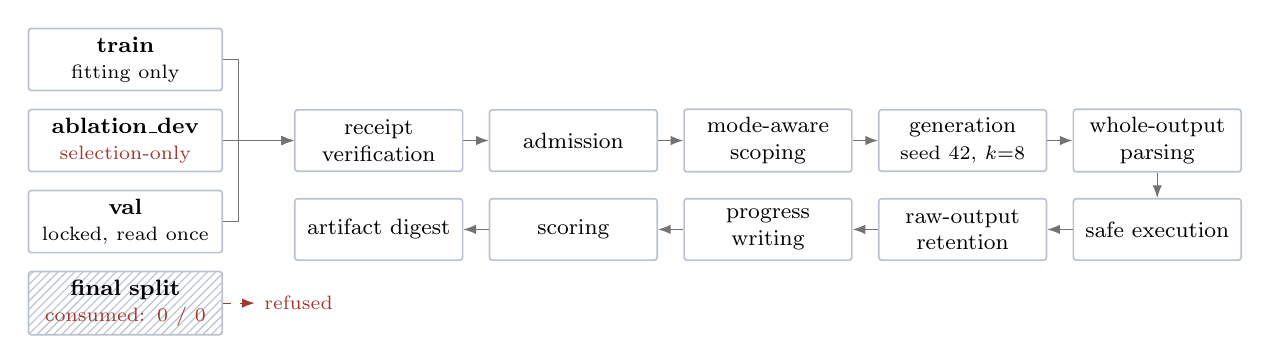
\begin{tikzpicture}[
  font=\footnotesize,
  st/.style={draw=orule,line width=0.6pt,rounded corners=1pt,
             text width=1.92cm,align=center,inner sep=3pt,minimum height=0.78cm},
  sp/.style={draw=orule,line width=0.6pt,rounded corners=1pt,
             text width=2.25cm,align=center,inner sep=3pt,minimum height=0.72cm},
  a/.style={-{Latex[length=1.6mm]},draw=black!55}
]
% splits
\node[sp] (train) {\textbf{train}\\\scriptsize fitting only};
\node[sp,below=2.2mm of train] (dev)
  {\textbf{ablation\_dev}\\\scriptsize \textcolor{ofail}{selection-only}};
\node[sp,below=2.2mm of dev] (val)
  {\textbf{val}\\\scriptsize locked, read once};
\node[sp,below=2.2mm of val,pattern=north east lines,pattern color=orule]
  (test) {\textbf{final split}\\\scriptsize \textcolor{ofail}{consumed: 0 / 0}};

% pipeline
\node[st,right=9mm of dev] (rcpt) {receipt verification};
\node[st,right=3.2mm of rcpt] (adm) {admission};
\node[st,right=3.2mm of adm] (scope) {mode-aware scoping};
\node[st,right=3.2mm of scope] (gen) {generation\\\scriptsize seed 42, $k{=}8$};
\node[st,right=3.2mm of gen] (parse) {whole-output parsing};
\node[st,below=3.2mm of parse] (exec) {safe execution};
\node[st,left=3.2mm of exec] (raw) {raw-output retention};
\node[st,left=3.2mm of raw] (prog) {progress writing};
\node[st,left=3.2mm of prog] (score) {scoring};
\node[st,left=3.2mm of score] (dig) {artifact digest};

\draw[a] (train.east) -- ++(2mm,0) |- (rcpt.west);
\draw[a] (dev.east) -- (rcpt.west);
\draw[a] (val.east) -- ++(2mm,0) |- (rcpt.west);
\draw[a,draw=ofail,dashed] (test.east) -- ++(4mm,0)
  node[right,font=\scriptsize,text=ofail] {refused};
\draw[a] (rcpt) -- (adm);
\draw[a] (adm) -- (scope);
\draw[a] (scope) -- (gen);
\draw[a] (gen) -- (parse);
\draw[a] (parse) -- (exec);
\draw[a] (exec) -- (raw);
\draw[a] (raw) -- (prog);
\draw[a] (prog) -- (score);
\draw[a] (score) -- (dig);
\end{tikzpicture}
\caption{Evaluation workflow and split roles. The rehearsal (Section~\ref{sec:rq4})
executes this entire chain on the permitted panel and is an operational check of
execution fidelity, \textbf{not} model selection. For the consumed split we give
neither size, membership, record counts nor any performance score; the two zeros
shown record the historical fact that the authorized attempt generated zero
candidates and zero reportable metrics.}
\label{fig:workflow}
\end{figure*}

\subsection{Predeclared decision rule}

Before either locked arm ran, a promotion rule was frozen in a hash-bound
receipt. Criterion~1 required \emph{all} of: \killk{8} gain $\geq +3.0$ points,
net gain $\geq 15$ functions, and exact two-sided McNemar $p < 0.01$. Further
criteria bounded permitted regression in reference validity, parse and execution
validity, and candidate diversity. Fixing the threshold beforehand is what makes
the outcome reported in Section~\ref{sec:rq1} interpretable.

\section{RQ1: Selection Inflation}
\label{sec:rq1}

Table~\ref{tab:main} and Figure~\ref{fig:devvslocked} give the answer. On the
selection panel, \killk{8} rose from $0.605166$ to $0.695572$, a gain of $9.04$
points. On the locked split the same checkpoint gave $0.628798$ against
$0.594452$: $+3.4346$ points, roughly $2.6\times$ smaller.

\begin{table}[t]
\caption{Main results. The two blocks are not comparable quantities.}
\label{tab:main}
\centering
\footnotesize
\begin{tabular}{@{}llrrr@{}}
\toprule
Panel & Arm & \killk{8} & Fns & Wilson 95\% \\
\midrule
\multicolumn{5}{@{}l}{\textit{Development --- selection-only, $n = 542$}}\\
& base   & 0.605166 & 328 & [0.5634, 0.6454] \\
& A@150  & 0.690037 & 374 & [0.6499, 0.7275] \\
& A@431  & 0.695572 & 377 & [0.6556, 0.7328] \\
& B@150  & 0.658672 & 357 & [0.6178, 0.6973] \\
\midrule
\multicolumn{5}{@{}l}{\textit{Locked validation --- not used for selection, $n = 757$}}\\
& base   & 0.594452 & 450 & [0.5591, 0.6289] \\
& A@431  & 0.628798 & 476 & [0.5938, 0.6625] \\
\midrule
\multicolumn{5}{@{}l}{\textit{Paired locked difference}}\\
& gained / lost / net & \multicolumn{3}{r}{$+114$ / $-88$ / $+26$} \\
& killed by both / neither & \multicolumn{3}{r}{$362$ / $193$} \\
& \killk{8} delta & \multicolumn{3}{r}{$+3.4346$ points} \\
& McNemar exact two-sided $p$ & \multicolumn{3}{r}{$0.0783$} \\
& predeclared requirement & \multicolumn{3}{r}{$p < 0.01$ --- \textbf{not met}} \\
& decision & \multicolumn{3}{r}{\textbf{retain base model}} \\
\bottomrule
\end{tabular}
\end{table}

\begin{figure}[t]
\centering
% Coordinates map Kill@8 v to x = (v - 0.50) * 25 cm.
% Every value below is taken verbatim from the receipts; see the package
% data file kill_at_8.csv, which carries its source digests.
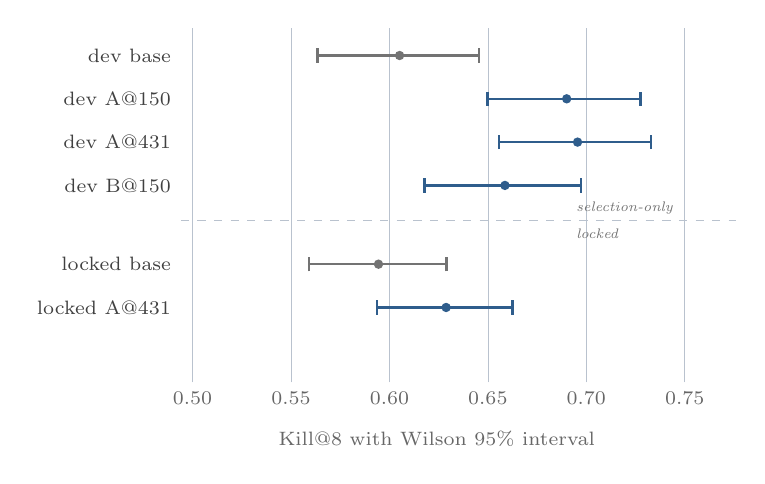
\begin{tikzpicture}[font=\scriptsize,x=1cm,y=1cm]
  % grid and axis
  \foreach \v/\lx in {0.50/0, 0.55/1.25, 0.60/2.5, 0.65/3.75, 0.70/5.0, 0.75/6.25}{
    \draw[orule,very thin] (\lx,-0.35) -- (\lx,4.15);
    \node[below,text=black!60] at (\lx,-0.35) {\v};
  }
  \node[below,text=black!60] at (3.1,-0.85) {\killk{8} with Wilson 95\% interval};

  % rows: {y}/{label}/{lo}/{point}/{hi}/{colour}
  \foreach \y/\lab/\lo/\pt/\hi/\c in {%
    3.80/{dev base}/1.585/2.629/3.636/black!55,
    3.25/{dev A@150}/3.747/4.751/5.688/oaccent,
    2.70/{dev A@431}/3.889/4.889/5.821/oaccent,
    2.15/{dev B@150}/2.944/3.967/4.934/oaccent,
    1.15/{locked base}/1.477/2.361/3.222/black!55,
    0.60/{locked A@431}/2.345/3.220/4.062/oaccent}{
      \draw[\c,line width=0.9pt] (\lo,\y) -- (\hi,\y);
      \draw[\c,line width=0.9pt] (\lo,\y-0.09) -- (\lo,\y+0.09);
      \draw[\c,line width=0.9pt] (\hi,\y-0.09) -- (\hi,\y+0.09);
      \fill[\c] (\pt,\y) circle (1.7pt);
      \node[left,text=black!75] at (-0.15,\y) {\lab};
  }
  \draw[orule,dashed] (-0.15,1.70) -- (6.9,1.70);
  \node[right,text=black!55,font=\tiny] at (4.75,1.86)
    {\textit{selection-only}};
  \node[right,text=black!55,font=\tiny] at (4.75,1.54)
    {\textit{locked}};
\end{tikzpicture}
\caption{Development and locked \killk{8} with Wilson 95\% intervals. The locked
pair (bottom two rows) is \textbf{positive but not significant} under the
predeclared $p < 0.01$ rule; its intervals overlap. Development and locked rows
measure different populations and must not be subtracted.}
\label{fig:devvslocked}
\end{figure}

The shrinkage is what selection bias predicts: the development panel chose the
checkpoint it then scored. The locked figure is positive, and it is the only
generalization estimate here.

It is equally important what the locked figure does not establish. With $202$
discordant pairs ($114$ versus $88$), an exact two-sided McNemar test
\cite{mcnemar1947note,dietterich1998tests} yields $p = 0.0783$ against a
required $p < 0.01$. The data are insufficient to conclude an effect at the
standard fixed in advance. That is not the same as concluding there is no effect
\cite{wasserstein2016asa,amrhein2019retire}, and we make no such claim. The
question is undetermined at this sample size and cannot be resolved by
re-measuring this split, which has now been used to decide.

\section{RQ2: Kill Rate Against Candidate Validity}
\label{sec:rq2}

Table~\ref{tab:validity} shows the trade-off. Reference validity fell from
$0.452114$ to $0.333388$ on the locked comparison, a $-11.8726$ point change,
and targets with \emph{any} reference-valid candidate fell from $675$ to $566$.
Over the same comparison parse validity rose $0.1486$ points and execution
validity rose $1.3870$ points.

\begin{table}[t]
\caption{Candidate validity. The regression is specific to reference validity;
parse and execution validity improved.}
\label{tab:validity}
\centering
\footnotesize
\begin{tabular}{@{}llrrrr@{}}
\toprule
Panel & Arm & Parse & Exec. & \textbf{Ref.} & Fns ref-valid \\
\midrule
\multicolumn{6}{@{}l}{\textit{Development --- selection-only}}\\
& base  & 0.983395 & 0.948570 & \textbf{0.565498} & --- \\
& A@150 & 0.997463 & 0.975092 & \textbf{0.458487} & --- \\
& A@431 & 0.998155 & 0.993081 & \textbf{0.455028} & --- \\
& B@150 & 0.998155 & 0.973478 & \textbf{0.448801} & --- \\
\midrule
\multicolumn{6}{@{}l}{\textit{Locked validation}}\\
& base  & 0.987285 & 0.928336 & \textbf{0.452114} & 675 \\
& A@431 & 0.988771 & 0.942206 & \textbf{0.333388} & 566 \\
& delta & $+0.1486$ & $+1.3870$ & $\mathbf{-11.8726}$ & $-109$ \\
\bottomrule
\end{tabular}
\end{table}

Three observations. First, the direction is consistent across all four
development arms, so it is a property of this supervision family rather than of
one checkpoint. Second, because parse and execution validity \emph{improved},
the regression is not explained by malformed or non-running code --- the tuned
model produces more usable tests that are more often wrong about the reference.
Third, the structural explanation is available and testable: kill rate credits
any candidate that separates mutant from reference, and a test that fails both
separates neither, but a test that fails the reference while failing the mutant
differently can still be credited. A validity-blind objective therefore admits
solutions a practitioner would reject.

We report this as an observed association under one recipe. We did not ablate
the objective, and we do not claim the trade-off is unavoidable.

\section{RQ3: Interpretability of Reported Numbers}
\label{sec:rq3}

\paragraph{Parsing semantics are part of the measurement}
Candidate extraction supports taking the first assertion or the whole output.
These score different artifacts. An earlier version of our final-run path never
set the mode explicitly and would have inherited a legacy default, producing a
plausible number under one parser while the frozen record named another. Parsing
mode belongs in the frozen protocol beside the seed.

\paragraph{Raw-output retention makes results auditable}
Every candidate slot retains its raw model output and a digest. This permitted
an independent recomputation of all $4{,}336$ digests in the rehearsal, and it
lets a disputed score be re-examined without regeneration. Pipelines that store
only verdicts cannot separate a scoring bug from a model behaviour after the
fact.

\paragraph{Split isolation must be structural}
Split roles are meaningful only if code cannot reach the wrong split. Our
final-split guard gated on \emph{authorization} --- a fact that, once recorded,
never expires --- rather than on whether anything remained to measure. A
permission check is not an exhaustion check, and the distinction cost us a
split.

\paragraph{Leakage}
Where targets come from public benchmarks, a model may recall an assertion
rather than derive one \cite{yang2023rephrased,kapoor2023leakage,liu2023evalplus}.
We classify assertion \emph{form} separately from assertion \emph{value} so that
a gain cannot be credited to the wrong mechanism, and we exclude records of one
execution mode from every rate because no validated evaluator exists for them.

\section{RQ4: Full-Scale Rehearsal}
\label{sec:rq4}

\subsection{The consumed measurement}

A one-time final measurement was authorized and attempted. It reached
\texttt{failed\_after\_authorization}: the single-use authorization was spent and
the run raised while admitting records. It produced \textbf{zero candidates and
zero reportable metrics}. Nothing was generated and nothing was scored. The
split is consumed and may never be rerun; a split that has been opened is no
longer held out regardless of what it produced.

The cause was a record-admission rule requiring a fixed field set to be
non-empty on \emph{every} record in a split, raising before returning any.
Records of one execution mode legitimately carry some of those fields blank, and
the established evaluator had always loaded the split and \emph{then} scoped
scoring by mode. The final path inverted that order and refused exactly the
records the pipeline was always going to exclude. The rejection reproduces
immediately on permitted splits, at no cost. A mode-only exemption would still
have been wrong: on the locked split, three records of the \emph{scored} mode
also carry one such field blank and were measured.

\subsection{Design and outcome of the rehearsal}

We rebuilt admission to partition by execution mode \emph{first} and apply field
requirements only to records that will be scored, importing the mode semantics
from the established evaluator rather than restating them. We then executed the
entire chain of Figure~\ref{fig:workflow} at full scale on the permitted panel,
under a hash-bound receipt whose source bindings are verified before the model is
loaded.

Table~\ref{tab:rehearsal} reports the outcome. The decisive figure is that
\killk{8} came out at $0.605166$, identical to the previously recorded value for
the same model on the same panel under the same evaluation-scope digest.

\begin{table}[t]
\caption{Operational rehearsal. Evidence of execution fidelity only.}
\label{tab:rehearsal}
\centering
\footnotesize
\begin{tabular}{@{}lr@{}}
\toprule
Quantity & Value \\
\midrule
Requested records & 594 \\
Scored targets (function mode) & 542 \\
Excluded by mode & 52 \\
Admission errors & 0 \\
Candidates ($542 \times 8$) & 4{,}336 \\
Generation batches $\times$ size & $271 \times 2$ \\
Raw outputs retained / digests & 4{,}336 / 4{,}336 \\
Missing / mismatched & 0 / 0 \\
Independently recomputed mismatches & 0 \\
Parse failures & 72 \\
Execution failures & 223 \\
Timeouts & 43 \\
Prompt-budget failures & 0 \\
Wall time / exit status & 577.753\,s / 0 \\
Weights written & 0 \\
\midrule
\killk{8} & \textbf{0.605166} \\
Prior recorded value & \textbf{0.605166} (exact match) \\
\bottomrule
\end{tabular}
\end{table}

\textbf{The scope of this result must be stated precisely.} It is evidence that
the rebuilt path computes the same number as the path that produced the
historical value. It is \emph{not} a model-performance result, \emph{not} a
generalization estimate, \emph{not} a selection result, \emph{not} a comparison
against any baseline tool, and \emph{not} a replacement for the lost
measurement. The rehearsal receipt carries
\texttt{final\_test\_measurement: false},
\texttt{eligible\_for\_model\_selection: false} and
\texttt{supports\_performance\_claim: false} as machine-checkable fields, and
the runner refuses a receipt lacking them.

\section{Discussion}

\paragraph{For practitioners scoring LLM test generators}
Report a validity metric beside the kill rate. The regression we measured is
invisible to a kill-rate-only report and moves opposite to the headline, so a
tool selected on kill rate alone may be selected against test quality.

\paragraph{For anyone using a held-out split once}
Execute the full path on permitted data at full scale before the irreversible
run. A smoke test on synthetic records proves the generator, not the pipeline.
Make the one-time authorization two-phase so a post-open failure does not consume
the split, and gate on exhaustion rather than permission.

\paragraph{On thresholds}
A predeclared threshold is uncomfortable precisely when it binds. Our
$p = 0.0783$ was close enough to $0.01$ that any rule written afterwards would
have been suspect. Fixing it in a hashed artifact before the run is what makes
the retention decision reportable at all.

\section{Threats to Validity}

\paragraph{Construct}
\killk{k} credits any distinguishing candidate, including a universally failing
test; we therefore report reference validity beside it. Mutants are an imperfect
proxy for real faults \cite{just2014mutants,papadakis2018mutationscores}.

\paragraph{Internal}
One locked criterion failed through a defect of ours: an adapter-specific digest
was placed inside a contract required to be identical across arms, which no
base/adapter pair can satisfy. We record it as a failure rather than
reinterpreting it; the decision does not rest on it because the significance
criterion failed independently. All development arms ran under one contract and
one scope digest, recorded identical, removing protocol drift as an explanation.

\paragraph{External}
One model, one parameter scale, one corpus, one supervision family, one seed. We
do not claim the shrinkage ratio or the validity trade-off transfers. Records of
one execution mode are excluded from every rate, so no claim is made about that
target class, and no native repository-level kill rate exists.

\paragraph{Statistical conclusion}
A single paired test on 202 discordant pairs. We report an exact test and Wilson
intervals \cite{wilson1927probable,arcuri2014hitchhiker} and avoid converting a
non-significant result into a null claim.

\paragraph{Reproducibility}
The consumed split cannot be reproduced by anyone. Everything else is
reproducible from committed receipts; the rehearsal is direct evidence, having
reproduced a prior value exactly.

\section{Replication Package}
\label{sec:replication}

An anonymized replication package accompanies this submission. Every numeric
value in this paper is traceable to one of the following receipts by SHA-256.
Paths are relative to the package root; no host, account or repository URL is
included, in keeping with double-anonymous review.

\begin{table}[h]
\caption{Receipted artifacts. Digests are truncated for space; full values are
in the package manifest.}
\label{tab:artifacts}
\centering
\scriptsize
\begin{tabular}{@{}ll@{}}
\toprule
Artifact & SHA-256 (prefix) \\
\midrule
Frozen development evaluation receipt & \texttt{062774028693cfcb} \\
Development selection receipt & \texttt{0188324fe9eb2a51} \\
Locked-validation preflight (rule frozen) & \texttt{97be6855d41b1186} \\
Locked-validation result receipt & \texttt{f7cdf84df8e65c51} \\
Rehearsal receipt (pre-run freeze) & \texttt{bae9510218641b67} \\
Rehearsal execution receipt (sanitised) & \texttt{06aca918d2821a1f} \\
\bottomrule
\end{tabular}
\end{table}

The package includes: the frozen protocol definition and its digest; the
promotion rule as committed before the locked run; per-arm metric receipts for
both panels; the rehearsal receipt and execution receipt; per-figure data files,
each carrying the digest of its source receipt in a header comment; and a
command list that re-derives every table from the receipts alone.

Raw generated outputs are retained but excluded from the package: they comprise
$4{,}336$ model completions for the rehearsal alone. Their individual digests are
published, so any retained output can be verified without redistribution. No
material from the consumed split is included, and none exists.

\section{Conclusion}

A $9.04$ point development-panel gain corresponded to $+3.4346$ points on a
locked split, which did not meet a predeclared significance threshold; the
untrained base model was retained. Over the same comparison, candidate reference
validity fell $11.8726$ points while parse and execution validity improved ---
a trade-off a kill-rate-only evaluation cannot see. A receipt-bound full-scale
rehearsal on a permitted split reproduced a prior measurement exactly,
establishing execution fidelity for the pipeline without touching a split that
had already been consumed by a failed one-time attempt.

The measurement practices that made these statements possible are cheap
individually and only valuable together: freeze the rule, bind the sources by
digest, retain raw outputs, keep split roles structural, and run the whole path
on permitted data before anything irreversible depends on it.

\bibliographystyle{IEEEtran}
\bibliography{references}

\end{document}
